\documentclass{amsbook}
\usepackage{../HBSuerDemir}
\usepackage[utf8x]{inputenc}  
\usepackage{graphicx}
\usepackage{wrapfig}
\usepackage[]{enumerate}

\begin{document}
    \hPage{b1p2/311}
    \renewcommand{\headrulewidth}{0pt}

    \begin{enumerate}[1)] \itemsep2pt
        \setcounter{enumi}{2}
        \item{If necessary, determine the interval of increase and decrease for r.}\\

        \item {$Determination\; of\;  asymptotes: $In polar coordinates one distinguishes two kinds of asymptotes as $circle-asymptote$ (in particular a point-asymptote as a degenerate case) and a $lineasymptote$.}\\
        \begin{figure} [htbp]
            \begin{center}
                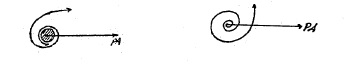
\includegraphics[width=300]
	            {images/b1p2-311-fig01-fig02.jpg}
            \end{center}
        \end{figure}
        \underline{Circle-asymptote}: It exists when $r \to a $ as $\theta \to \infty$.\\
        \underline{Line-asymptote}: (When necessary):\\

        \hspace{1cm}The direction of a line asymptote exists when $r \to \infty$ as $\theta \to \theta_o$. If $l$ is such an asymptote
        (See Fig.), its normal equation will be\\
        \begin{minipage}[c]{0.45\textwidth}
            \begin{itemize}\itemsep2pt
                \noindent
                $rcos(\theta - \alpha)-p=0 $ \\ 

                where \\ 

                \hspace{1cm}$\alpha = \theta_o +  {\pi}/{2}$ \\

                \hspace{1cm}$p = \lim_{\substack{\theta \to \theta_o \\ (r \to \infty)}}(rsin(\theta - \theta_o)).$
            \end{itemize}
        \end{minipage}
        \hfill
        \begin{minipage}[c]{0.45\textwidth}
            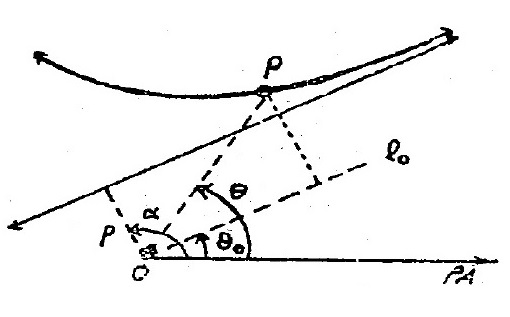
\includegraphics[width=\textwidth]{images/b1p2-311-fig03.jpg}
        \end{minipage}

        \hspace{1cm} Note that 
        $\theta_o =\ k\pi$ and $\theta_o =\ (2k+1) {\pi}/{2}$  correspond to horizontal and vertical asymptotes respectively.\\

        \item { \underline{Intercepts other than the pole}. For PA-intercepts one sets $\theta = k \pi$ and for CPA-intercepts $\theta =\ k\pi$ and $\theta_o =\ (2k+1) {\pi}/{2}$ in the equation. The curve passes through the pole when $r = 0$.}\\
    \end{enumerate}
    \noindent
    \underline{Example}. Sketch the curve of $r = 2 \ tan\theta$\\

    \noindent
    \underline{Solution}.\\

    \begin{enumerate}[1)]
        \item{ $D= (-\infty,\ +\infty) - \{\theta = (2k+1)\  \frac{\pi}{2} : k \in \mathbb{Z}\}  $ \\

        $\quad T = \pi \Rightarrow \; D_1 = (0, \pi) - \{ \pi / 2\} $}
    \end{enumerate}


\end{document}